\section{FOCUSA Backend}

% TODO: bibliography!!
The FOCUSA backend is one of the many deliverables our project delivers.
During design, the project was broken into multiple isolated, loosely coupled and horizontally scalable modules. 
Called the microservice architecture, this breaks code into small and manageable pieces which can be rapidly implemented and quickly tested.

Each microservice runs in a \textbf{highly isolated manner}, without needing to share any resources in common. The services do not need to share any memory, variables, or storage. 
\emph{How will services share data?} 
Services will use message passing over WebSockets, or simple RPC (over HTTP) when they need to communicate.

This architecture also supports \textbf{great scalability}. Each service can run on its machine (container, virtual, physical, or 
even geographical transparency) 
The same service can have multiple instances, independently governed by one or more load balancers.

Any communication with a microservice operates \textbf{over a stateless protocol}, like HTTP.
There isn't any specific full-duplex session maintenance mechanism in the TCP/IP suite, and thus a token must be attached to every packet. This token references a session. We observed a single point of failure when trying to solve session management by using a centralised service.

The approach we used was signing a \textbf{cryptographic token called a JWT (JSON Web Token)}. 
The authentication service plays the role of signing these tokens and sending them to the client with a "refresh cookie". The client then attaches this token to every future request made to any service in our project domain. It is possible because the JWT contains 
ALL the session data as a JSON payload, encrypted and entrusted to the client. None of the services (except the authentication service) store session data.

It is dangerous to trust the client with storing session data. \emph{Can a client generate a JSON payload on their own and impersonate a user?} No.~\cite{JWTBestPractices}

JWTs also contain a digital signature. However, similar to a session cookie, the services cannot distinguish between a valid client and a client impersonating a user solely using their JWTs. Since all our services depend on the session state written in the JWT, shared by the client, we carefully adhered to these rules for handling JWTs throughout development:

\begin{itemize}
    \item Every JWT has a validity window, after which it expires. Always keep this window small. 
    Keeping a small window means that a JWT quickly expires after its creation, thus preventing any malicious party from misusing the JWT for a long time.
    \item Every client also keeps a session refresh cookie used to regenerate a JWT after expiry. The client can use the refresh cookie to ask for a new JWT.
    \item The JWT is always kept in volatile storage. It helps avoid XSS attacks and localStorage stealing.
    \item Protect the JWT from being stolen. Also, reduce the risk of session hijacking if the JWT gets stolen.
\end{itemize}

Our approach uses an asymmetric-key digital signature standard called RS256. Here, the authentication service signs the JWT using a private key. The other services keep the public key. This way, any service can verify the signature of the JWT shared by the client. The other services will only accept the JWT when signed by the authentication service. 
Failure to provide a valid JWT will lead to an intentional Denial of Service since the service will assume a malicious user is playing with the system.

As listed in the Design chapter, the FOCUSA backend contains the following major services:
\begin{itemize}
    \item \textbf{Auth:} performs the authentication process based on a username-password pair, and returns refresh cookies with a JWT.
    \item \textbf{Roles:}  returns the roles that a user belongs to. It depicts the different roles that different admins perform.
    \item \textbf{Profiles:} Each user has a unique profile, containing details like the user display picture, username, and the various courses the user has subscribed to.
    \item \textbf{Courses:}  returns the details of the courses which includes the course title and the different users subscribed to the course, as well as a provision for new users to subscribe to the course. Only users with certain roles can moderate their respective courses.
    \item \textbf{Posts:} refers to posts posted by the course moderators. The moderators can perform CRUD operations on these posts.
    \item \textbf{Notifications:}  sends notifications to the user devices and also monitors the database for changes.
    \item \textbf{Storage:} performs all functions related to file upload, download, and streaming.
\end{itemize}

The following sections will describe our workflow and an overview of our deployment strategy.

\subsection{Workflow}

Every service in the FOCUSA backend has three major layers:
\begin{itemize}
    \item \textbf{DAO}, which includes a set of functions regarding Database, Analytics and Operations. 
    These functions are invoked and executed on call at the next stage.
    \item \textbf{REST API}, which acts as a thin ExpressJS layer between the main API gateway and the DAO.
    This layer performs RPC-based communication with proper JWT verification checks.
    \item \textbf{GraphQL API gateway integration}, where the microservices are integrated, over a graph query language gateway.
    GraphQL API allows the developer to build surprisingly advanced systems using resolvers that invoke the REST API services.
    The GraphQL API gateway also supports queries, mutations, and subscriptions. This allows us to build practically any front-end, which supports the typical query-response RPC-based mechanism, and also the more complex message-based notification mechanism.
\end{itemize}

\begin{figure}[h!]
    \begin{center}
        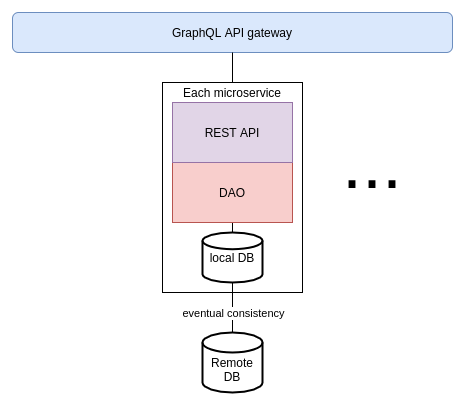
\includegraphics[width=8cm]{Microservice.png}
    \end{center}
    \caption{Our layered approach to building each microservice.}
    \label{fig:microservice}
\end{figure}

All microservices were built in three layers, as shown in \ref{fig:microservice}, following this layered architecture for each service. 

It is important to note that our notification service uses a pull-notification technique. It uses a 
publisher-subscriber architecture which only transfers a digest of messages whenever the client asks for them. Unlike polling, 
this system operates on an event loop.

\subsection{Deployment}

Initially, we had decided to deploy it on the Heroku cloud. Heroku provides virtual containers called dynos. Each free tier dyno by itself has very few resources allocated to it. An account is allowed to operate multiple dynos. Each service ran very efficiently, 
with latencies as low as 70ms per request.

This strategy quickly hit a roadblock when we noticed that data isn't persisting at the dynos~\cite{HerokuActiveStorage}. 
Heroku provides ephemeral storage to dynos. The data is volatile and gets purged/reallocated after inactivity.
We need to integrate custom AWS S3 storage to the dyno if we want persistent storage. 

We ultimately decided to operate on self-hosted Docker containers. Docker was easier to customize. The only issue with self-hosting is server availability. Hosting on AWS services is a long-term goal.